\section{Implementation}
\label{sec:implementation}

\begin{figure}[t]
  \centering
    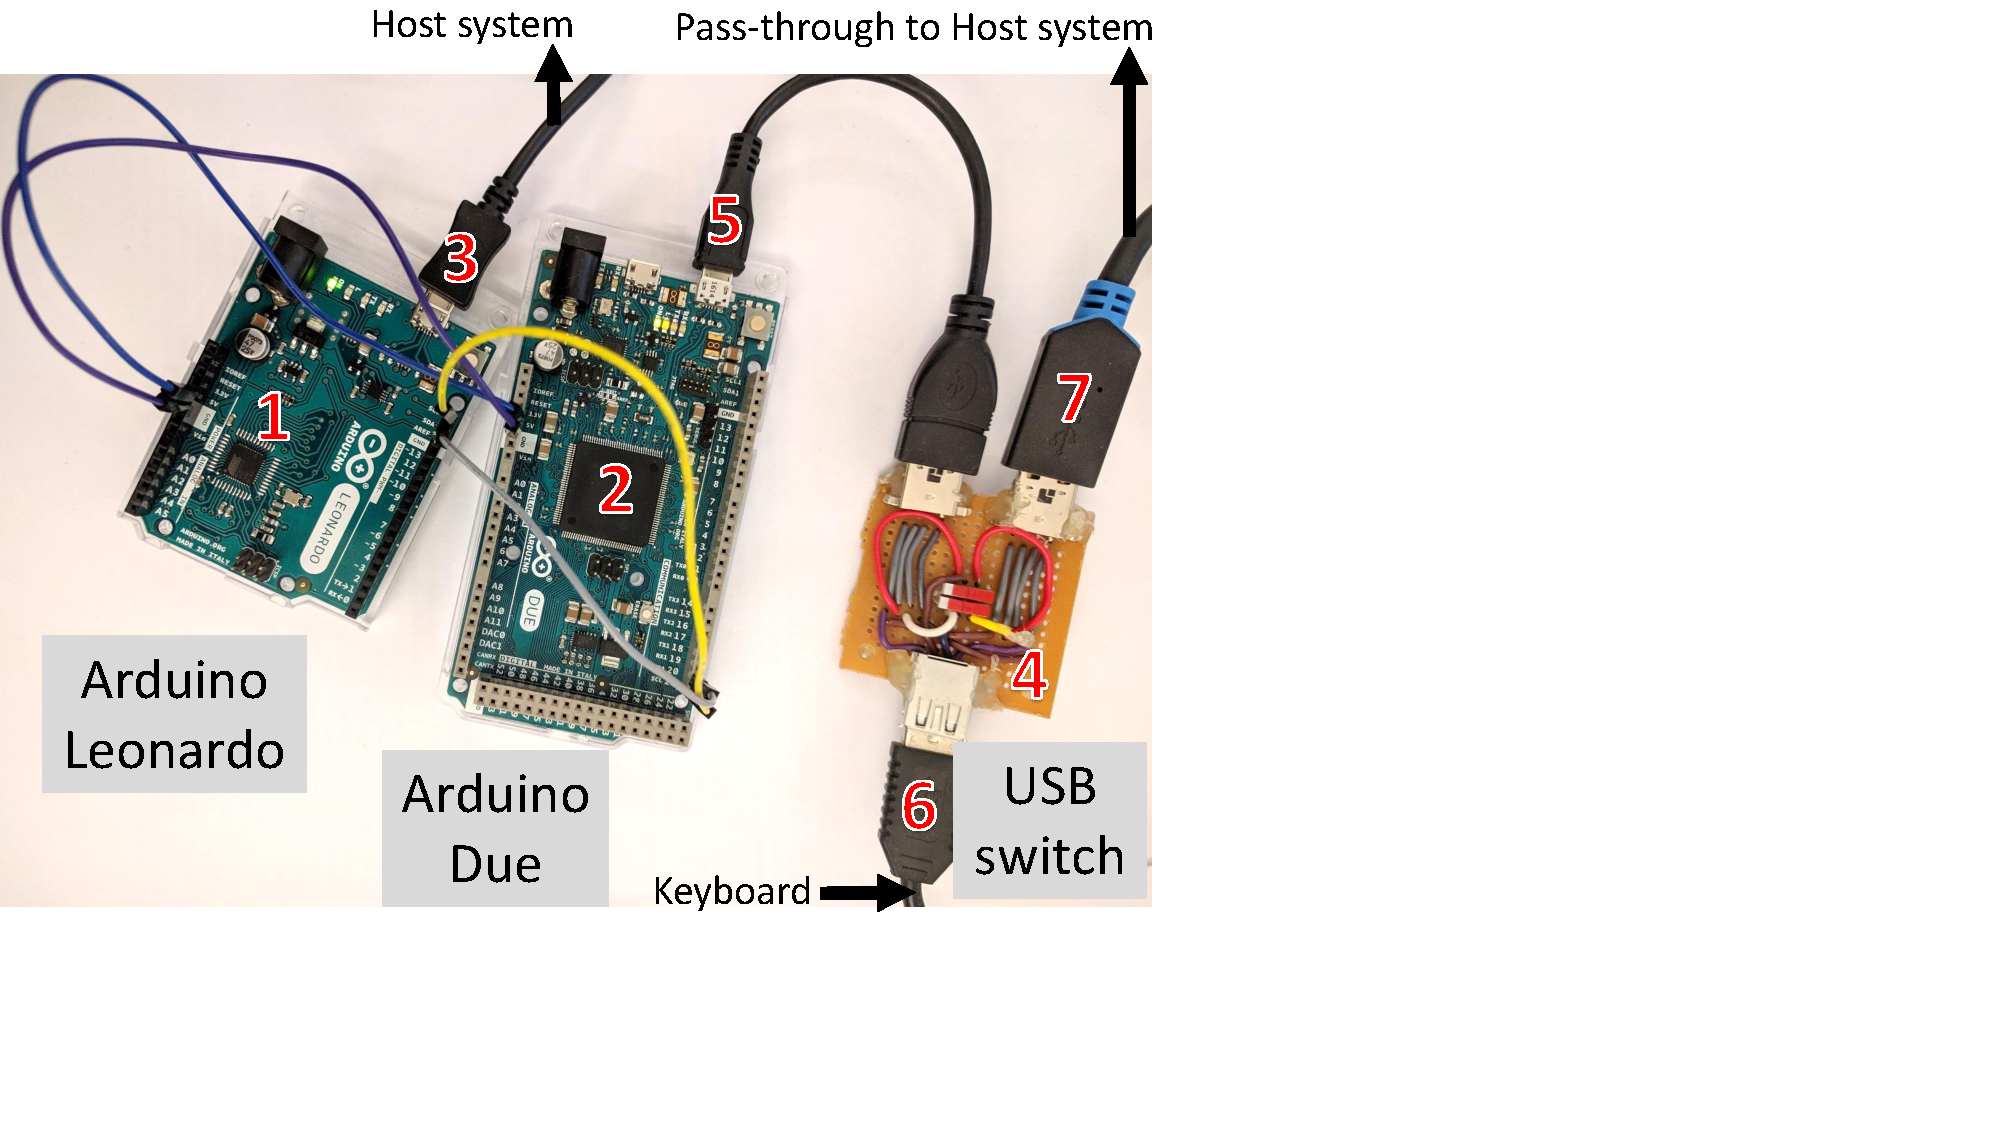
\includegraphics[trim={0 2.5cm 14cm 0}, clip, width=0.5\linewidth]{setup4_revised.pdf}
    \caption{\textbf{\device prototype.} \device prototype consists of the following: 1) Arduino Due board is connected with the keyboard and executes cryptographic operations in \tls, 2) Arduino Leonardo board communicates with the browser using \webusb, 3) \usb connection from the \device to the host system, 4) \usb switch to switch between the secure and insecure mode (pass-through), 5) the connection between the \device and the \usb switch, 6) the keyboard connection, 7) the host pass-through connection for the insecure mode.}
    %\vspace{-10pt}
    \label{fig:setup}
\end{figure}

We implemented a complete \name system. Our implementation consists of three parts: (1) \device prototype, (2) \server input trace matching library and (3) \tool UI analysis tool. 

\subsection{\device Prototype} 

Our \device prototype consists of two Arduino boards and one USB switch, as shown in Figure~\ref{fig:setup}. We used two separate boards, and an additional switch, because of the limited USB interfaces and computational power in the used Arduino boards, but we emphasize that a production device could be realized as a single embedded device
%\footnote{Two boards were used due to a limitation of the older \webusb driver that only supported AVR based microcontroller such as Arduino Leo which is not sufficient to execute cryptographic operations. We already developed a limited version of the same prototype on a single Arduino Zero board using the newer driver to evaluate the viability of a single board.}. 
In more detail, our \device prototype consists of an Arduino Leonardo board, a $16$ MHz AVR microcontroller, which communicates with the host using \webusb, and an Arduino Due, an $84$ MHz ARM Cortex-M3 microcontroller, to execute computationally more expensive cryptographic operations needed for \tls. The two boards are connected using the $I^2C$ protocol~\cite{i2c} in the master-slave configuration. The prototype can be connected to the keyboard via a custom-made USB switch (see $4$ in Figure~\ref{fig:setup}). We use two boards as the \webusb library we used only supported AVR boards such as Arduino Leonardo which is not powerful enough to execute cryptographic operations required by the \tls that we implement on the Arduino Due board. We already developed a limited version of the same prototype on a single Arduino Zero board using the newer driver to evaluate the viability of a single board.

As the currently available version of the \webusb library \cite{webusb} allows only one \usb interface, our prototype cannot emulate a keyboard (interrupt transfer) and a persistent data (bulk transfer) device required for the \tls channel at the same time. Therefore, our prototype sends keyboard signals to the \js code running in the browser. The \js code interprets these signals and translates them to keyboard input on the web page.
We use the Arduino cryptographic library for the \tls. The limited set of cipher suites in our \tls implementation uses 128-bit AES (CTR mode), Ed25519 \& Curve25519 for signatures, Diffie-Hellman for key exchange and SHA256 for the hash function. Our prototype implementation is approximately 2.5K lines of code. 


\subsection{\server Implementation} 

Our server implementation for input trace matching is a \java EE Servlet hosted on an Apache Tomcat web server. We tested this implementation on a standard server platform, but the same code could be installed on a PLC server, such as~\cite{controlbyweb,siemens,siemens2,schneider}, as well. If a legacy PLC server does not allow installation of new code, our system could be deployed via a proxy, as discussed in Section~\ref{sec:discussion}. The server implementation consists of \js that is served to the host's browser. We develop this \js code that uses Google Chrome's \webusb API to communicate with the \device. We use \texttt{XMLHttpRequest} to communicate with the remote server. \server users \java cryptographic library to implement \tls. The input trace matching is computed on the server after it decrypts the trace data from the \tls channel. This implementation is approximately 500 lines of code.

 % \begin{figure}[t]
 %  \centering
 %  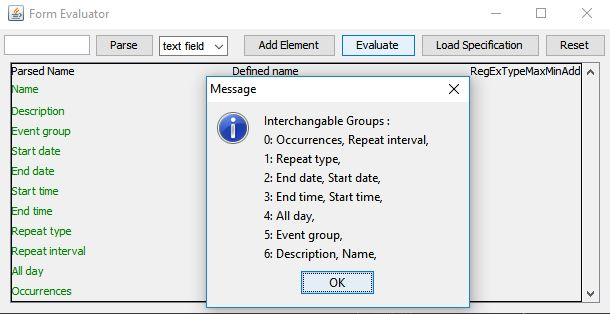
\includegraphics[width=0.6\linewidth]{IntegriTool.JPG}
 %  \caption{\textbf{\tool prototype.} A screenshot of \tool prototype that shows a parsed webpage specification and the groups of swappable input fields.} \vspace{-5pt}
 %  \label{fig:integriTool}
 % \end{figure}

\subsection{\tool Implementation} 

We implemented the UI analysis tool in \java based on the \java AWT graphics library. The tool is around 1.5K lines of code and uses the \java native XML interpreter library to read the specification, \textsc{dk.brics.automaton}~\cite{brics} for regular expression and \emph{Jsoup} \html parser to parse web pages. 
%An example snapshot of the \tool is depicted in Figure~\ref{fig:integriTool}.



